\section{Roteiro da Aula}

\begin{enumerate}

\item
Falar sobre produto escalar de dois vetores:

\[
 \vec A \, \cdot \vec B = |\vec A| \, |\vec B| \, \cos \theta
\]

\begin{figure}[htb]
    \centering
    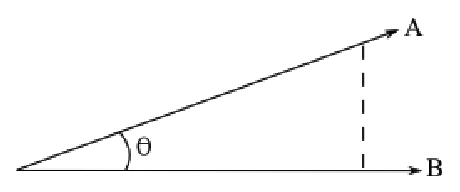
\includegraphics[scale=0.8]{capitulos/capitulo2/figuras/roteiro_da_aula1.eps}
    \caption{Produto escalar}
    \label{fig:roteiro_da_aula1}
\end{figure}

\[
 \vec A \, \cdot \vec B = \sum_{i=1}^N A_i \, B_i
\]

Se

\[
   \begin{array}{ll}
     \vec A \, \cdot \vec B = 0 & \Rightarrow \cos \theta = 0 \\
                                & \Rightarrow \theta = \displaystyle \frac{\pi}{2} + n\,\pi\,; \qquad n = 0, 1, \ldots \\
   \end{array}
\]

\begin{figure}[htb]
 \centering
 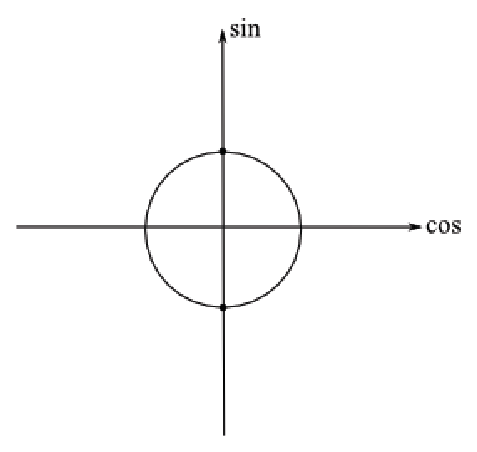
\includegraphics[scale=0.8]{capitulos/capitulo2/figuras/roteiro_da_aula2.eps}
 \caption{?}
 \label{fig:roteiro_da_aula2}
\end{figure}

dizemos que $\vec A$ e $\vec B$ são ortogonais.

\item
Estender a noção de ortogonalidade para funções

\begin{figure}[htb]
 \centering
 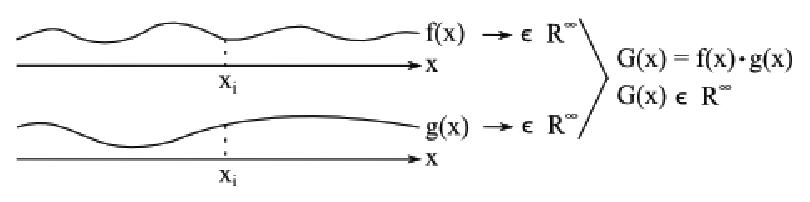
\includegraphics[scale=1.0]{capitulos/capitulo2/figuras/roteiro_da_aula3.eps}
 \caption{?}
 \label{fig:roteiro_da_aula3}
\end{figure}

\[
 \sum_i \, f\,(x_i) \, g\,(x_i) \equiv \sum_i \, G\,(x) \rightarrow \int \, f\,(x) \, g\,(x) \, dx = 0
\]

Se \esp{\int \, f\,(x) \, g\,(x) \, dx = 0} então $f(x)$ e $g(x)$ são ortogonais.

\item
Base de vetores ortogonais e polinômios ortogonais como base do espaço de polinômios. Mostrar que se um polinômio $P_{x}$ é ortogonal aos polinômios da base, então ele é perpendicular a todos os polinômios do espaço.

\begin{figure}[htb]
 \centering
 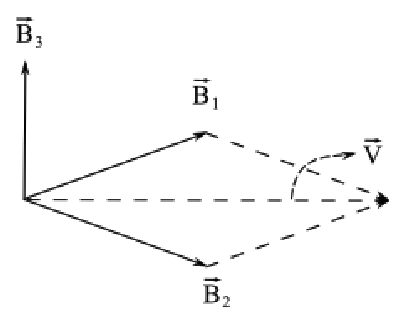
\includegraphics[scale=0.8]{capitulos/capitulo2/figuras/roteiro_da_aula4.eps}
 \caption{?}
 \label{fig:roteiro_da_aula4}
\end{figure}

\[
 \vec V = C_1 \, \vec B_1 + C_2 \, \vec B_2
\]

\[
 \left.
 \begin{array}{l}
  \vec B_3 \cdot \vec B_1 = 0 \\
  \vec B_3 \cdot \vec B_2 = 0
 \end{array}
 \right\}
 \Rightarrow
 \vec B_3 \cdot \vec V = 0
\]

\item
Mostrar a propriedade de ortogonalidade dos polinômios de Legendre

\[
 \int_{-1}^1 P_m\,(x) \, P_n\,(x)\,dx =
 \left\{
 \begin{array}{cl}
  0                & \qquad \mbox{para $n \neq m$} \\ \vspace*{0.2cm}
  \displaystyle \frac{2}{2\,n+1} & \qquad \mbox{para $m = n$}
 \end{array}
 \right.
\]

\item
Falar da interpolação de Lagrange

\textbf{Grau 1}

\begin{figure}[htb]
 \centering
 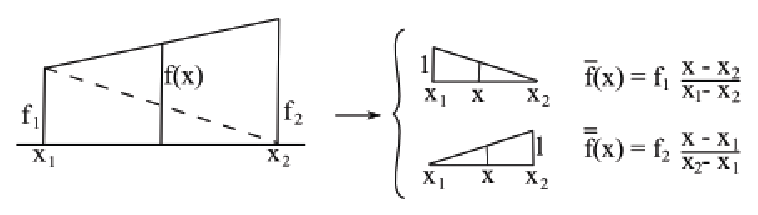
\includegraphics[scale=1.0]{capitulos/capitulo2/figuras/roteiro_da_aula5.eps}
 \caption{?}
 \label{fig:roteiro_da_aula5}
\end{figure}

\textbf{Grau 2}

\begin{figure}[htb]
 \centering
 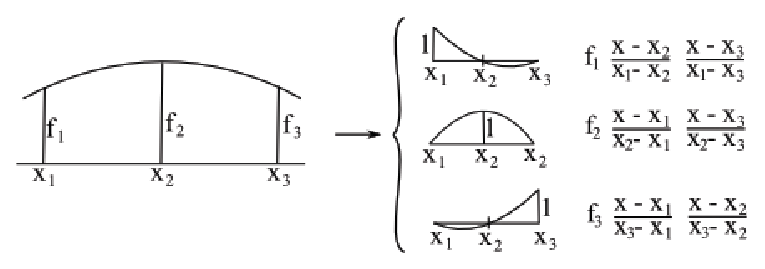
\includegraphics[scale=1.0]{capitulos/capitulo2/figuras/roteiro_da_aula6.eps}
 \caption{?}
 \label{fig:roteiro_da_aula6}
\end{figure}

Grau $n-1 \Rightarrow n$ pontos.

\end{enumerate}
